% Dados: aba Validações da planilha (registros por data de execução) e execução de 19/10/2026
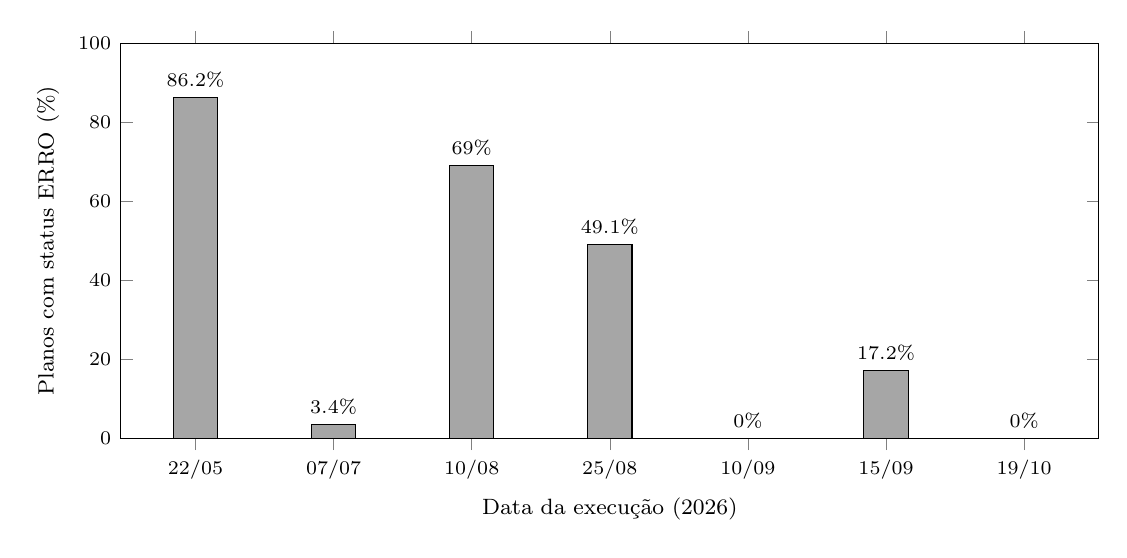
\begin{tikzpicture}
\begin{axis}[
  ybar,
  width=14cm, height=6.6cm,
  bar width=16pt,
  ymin=0, ymax=100,
  ylabel={Planos com status ERRO (\%)},
  symbolic x coords={22/05,07/07,10/08,25/08,10/09,15/09,19/10},
  xtick=data,
  xlabel={Data da execução (2026)},
  nodes near coords={\pgfmathprintnumber[fixed,precision=1]{\pgfplotspointmeta}\%},
  nodes near coords style={font=\scriptsize},
  ticklabel style={font=\scriptsize},
  label style={font=\footnotesize},
  enlarge x limits=0.09,
]
\addplot[fill=black!35, draw=black] coordinates {
  (22/05,86.2) (07/07,3.4) (10/08,69.0) (25/08,49.1) (10/09,0) (15/09,17.2) (19/10,0)};
\end{axis}
\end{tikzpicture}
